\documentclass[12pt]{article}
\usepackage{amsmath}
\usepackage{amssymb}
\usepackage{graphicx}
\usepackage{hyperref}
\usepackage{multicol}
\usepackage[latin1]{inputenc}
\usepackage{listings}
\usepackage{scrextend}

\usepackage{subcaption}

\title{ComS 342\\Recitation 2, 10:00 Tuesday\\Homework 2}
\author{Sean Gordon}
%\date{09/09/2019}

\begin{document}
\maketitle


%\begin{addmargin}[2.5em]{1.5em}
\noindent 1) $(+ (* 10\ 2) 1)$ and $(- (* 9\ 3) 6)$

\noindent 2)


\begin{figure}[h!]
  \centering
  \begin{subfigure}[b]{0.4\linewidth}
    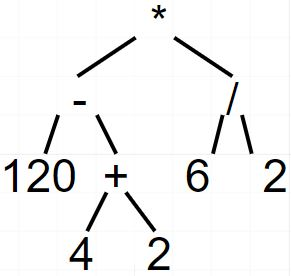
\includegraphics[width=\linewidth]{ComS342_HW2_2a.jpg}
    \caption{(* (- 120 (+ 4 2)) (/ 6 2))}
  \end{subfigure}
  \begin{subfigure}[b]{0.4\linewidth}
    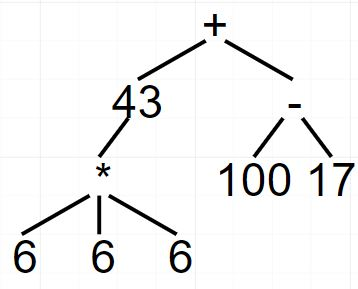
\includegraphics[width=\linewidth]{ComS342_HW2_2b.jpg}
    \caption{(+ 43 (* 6 6 6) (- 100 17))}
  \end{subfigure}
  \label{fig:Pt2}
\end{figure}





\noindent 3a) AST provides functions and helpers to work with the program, while Evaluator makes use of those functions to compute the result of the program. \\

\noindent b) Once the input is read, it is parsed into its respective parse tree by the Reader class. This tiered object is then passed to the Evaluator class. This object is passed around through various methods so the methods defined in Evaluator can climb the tree, evaluating as they go until the result is finally returned.\\
Assuming the interpreter reads $(+\ 1\  1)$ from the console, it will first parse the program into an $\textit{AddExp}$ containing two $\textit{\_val}$s (1 and 1).\\ 
It is then passed through Evaluator until it reaches the corresponding visit method for AddExp, where it loops through each operand and performs the addition operation.\\ 
This value is then returned up through the chain until it reaches interpreter once more and is printed to the screen.\\

c) The visitor pattern defined in AST.java is implemented in Evaluator.java as a set of functions that match with a given operator to work with its operands.\\ 
For example, if a DivExp operator is given with two operands, the values will be passed into the visit function with the DivExp parameter where the two operands will be divided.\\


4)...

5)...

%\end{addmargin}
\end{document}